\documentclass{article}
\usepackage[utf8]{inputenc}
\usepackage[english]{babel}
\usepackage[font=small,labelfont=bf]{caption}
\usepackage{geometry}
\usepackage{natbib}
\usepackage{pxfonts}
\usepackage{graphicx}
\usepackage{newfloat}
\usepackage{setspace}
%\doublespacing

\newcommand{\topics}{S1}
\newcommand{\corrmats}{S2}
\newcommand{\matchmats}{S3}
\newcommand{\featureimportance}{S4}
\newcommand{\listlearning}{S5}
\newcommand{\topicopt}{S6}


\title{How is experience transformed into memory?}
\author{Andrew C. Heusser, Paxton C. Fitzpatrick, and Jeremy R. Manning\\Department of Psychological and Brain Sciences\\Dartmouth College, Hanover, NH 03755, USA\\Corresponding author: jeremy.r.manning@dartmouth.edu}

\bibliographystyle{apa}

\begin{document}
\maketitle

\begin{abstract}
How our experiences unfold over time define unique \textit{trajectories} through the relevant representational spaces.  Within this geometric framework, one can compare the shape of the trajectory formed by an experience to that defined by our later remembering of that experience.  We propose a framework for mapping naturalistic experiences onto geometric spaces that characterize how they unfold over time.  New insights emerge when we apply this approach to a naturalistic memory experiment which had participants view and recount a video.  We found that the shapes of the trajectories formed by participants' recountings were all highly similar to that of the original video, but participants differed in the level of detail they remembered.  We also identified a network of brain structures that are sensitive to the ``shapes'' of our ongoing experiences, and an overlapping network that is sensitive to how we will later remember those experiences.
\end{abstract}


\section*{Introduction}

What does it mean to \textit{remember} something? In traditional episodic memory experiments \citep[e.g., list-learning or trial-based experiments;][]{Murd62a, Kaha96}, remembering is often cast as a discrete and binary operation: each studied item may be separated from the rest of one's experiences, and that item may be labeled as having been recalled versus forgotten. More nuanced studies might incorporate self-reported confidence measures as a proxy for memory strength, or ask participants to discriminate between ``recollecting'' the (contextual) details of an experience or having a general feeling of ``familiarity'' \citep{Yone02}. However, characterizing and evaluating memory in more realistic contexts (e.g., recounting a recent experience to a friend) is fundamentally different in at least three ways~\citep[also see][for a review]{KoriGold94}.  First, real world recall is continuous, rather than discrete.  Unlike in trial-based experiments, removing a (naturalistic) event from the context in which it occurs can substantially change its meaning.  Second, the specific words used to describe an experience have little bearing on whether the experience should be considered to have been ``remembered.''  Asking whether the rememberer has precisely reproduced a specific set of words to describe a given experience is nearly orthogonal to whether they were actually able to remember it.  In classic (e.g., list-learning) memory studies, counting the number or proportion of precise recalls is often a primary metric of assessing the quality of participants' memories.  Third, one might remember the \textit{gist} or essence of an experience but forget (or neglect to recount) particular details.  Capturing the gist of what happened is typically the main ``point'' of recounting a memory to a listener whereas, depending on the circumstances, accurate recall of any specific detail may be irrelevant.  There is no analog of the gist of an experience in most traditional memory experiments; rather we tend to assess participants' abilities to recover specific details (e.g., computing the proportion of specific stimuli they remember, which presentation positions the remembered stimuli came from, etc.).

How might one go about formally characterizing the gist of an experience, or whether that gist has been recovered by the rememberer?  Any given moment of an experience derives meaning from surrounding moments, as well as from longer-range temporal associations~\citep[e.g., ][]{LernEtal11}.  Therefore the timecourse of how an event unfolds is fundamental to its overall meaning.  Further, this hierarchy formed by our subjective experiences at different timescales defines a \textit{context} for each new moment~\citep[e.g., ][]{HowaKaha02, HowaEtal14}, and plays an important role in how we interpret that moment and remember it later~\citep[for review see][]{MannEtal15}.  Our memory systems can then leverage these associations to form predictions that help guide our behaviors~\citep{RangRitc12}.  For example, as we navigate the world, the features of our subjective experiences tend to change gradually (e.g.\ the room or situation we are in is strongly temporally autocorrelated), allowing us to form stable estimates of our current situation and behave accordingly~\citep{ZackEtal07, ZwaaRadv98}.  Although our experiences most often change gradually, they also occasionally change suddenly~\citep[e.g., when we walk through a doorway; ][]{RadvZack17}.  Prior research suggests that these sharp transitions (termed \textit{event boundaries}) during an experience help to discretize our experiences into \textit{events}~\citep{RadvZack17, BrunEtal18, HeusEtal18, ClewDava17, EzzyDava11, DuBrDava13}.  The interplay between the stable (within event) and transient (across event) temporal dynamics of an experience also provides a potential framework for transforming experiences into memories that distill those experiences down to their essence-- i.e., their gists.  For example, prior work has shown that event boundaries can influence how we learn sequences of items~\citep{HeusEtal18, DuBrDava13}, navigate~\citep{BrunEtal18}, and remember and understand narratives~\citep{ZwaaRadv98, EzzyDava11}.

Here we sought to examine how the temporal dynamics of a ``naturalistic'' experience were reflected in participants' later memories of that experience.  We analyzed an open dataset which comprised behavioral and functional Magnetic Resonance Imaging (fMRI) data collected as participants viewed and then verbally recalled an episode of the BBC television series \textit{Sherlock}~\citep{ChenEtal17}.  We developed a computational framework for characterizing the temporal dynamics of the moment-by-moment content of the episode (and of participants' verbal recalls).  Specifically, we use topic modeling~\citep{BleiEtal03} to characterize the thematic conceptual (semantic) content present in each moment of the episode and recalls, and we use Hidden Markov Models~\citep{Rabi89, BaldEtal17} to discretize the evolving semantic content into events.  In this way, we cast naturalistic experiences (and recalls of those experiences) as \textit{topic trajectories} that describe how the experiences evolve over time.  In other words, the episode's topic trajectory is a formalization of its gist.  Under this framework, successful remembering entails verbally ``traversing'' the topic trajectory of the original episode, thereby reproducing the gist of the original episode.  In addition, comparing the shapes of the topic trajectories of the original episode and of participants' retellings of the episode reveals which aspects of the episode were preserved (or lost) in the translation into memory.  We also identified a network of brain structures whose responses (as participants watched the episode) reflected the gist of the episode, and a second network whose responses reflected how participants would later recount the episode.


\section*{Results}
To characterize the gists of the \textit{Sherlock} episode participants watched and their subsequent recountings of the episode, we used a topic model~\citep{BleiEtal03} to discover the latent thematic content in the video.  Topic models take as inputs a vocabulary of words to consider and a collection of text documents; they return as output two matrices.  The first output is a \textit{topics matrix} whose rows are topics (latent themes) and whose columns correspond to words in the vocabulary. The entries of the topics matrix define how each word in the vocabulary is weighted by each discovered topic.  For example, a detective-themed topic might weight heavily on words like ``crime,'' and ``search.''  The second output is a \textit{topic proportions matrix}, with one row per document and one column per topic.  The topic proportions matrix describes which mix topics is reflected in each document.

\cite{ChenEtal17} collected hand-annotated information about each of 1000 (manually identified) scenes spanning the roughly 45 minute video used in their experiment.  This information included: a brief narrative description of what was happening; whether the scene took place indoors vs. outdoors; names of any characters on the screen; names of any characters who were in focus in the camera; names of characters who were speaking; the location where the scene took place; the camera angle (close up, medium, long, etc.); whether or not background music was present; and other similar details (for a full list of annotated features see \textit{Methods}).  We took from these annotations the union of all unique words (excluding stop words, such as ``and,'' ``or,'' ``but,'' etc.) across all features and scenes as the ``vocabulary'' for the topic model.  We then concatenated the sets of words across all features contained in overlapping 50-scene sliding windows, and treated each 50-scene sequence as a single ``document'' for the purposes of fitting the topic model.  Next, we fit a topic model with (up to) $K = 100$ topics to this collection of documents.  We found that 28 unique topics (with non-zero weights) were sufficient to describe the time-varying content of the movie (see \textit{Methods}; Figs.~\ref{fig:schematic}, \topics).  Note that our approach is similar in some respects to Dynamic Topic Models~\citep{BleiLaff06}, in that we sought to characterize how the thematic content of the episode evolved over time.  However, whereas Dynamic Topic Models are designed to characterize the how the properties of collections of documents change over time, our approach allows us to examine the topic dynamics within a single video.  Specifically, our approach yielded (via the topic proportions matrix) a single \textit{topic vector} for each timepoint of the episode (we set timepoints to match the acquisition times of the 1976 fMRI volumes collected as participants viewed the episode).

\begin{figure}[tp]
\centering
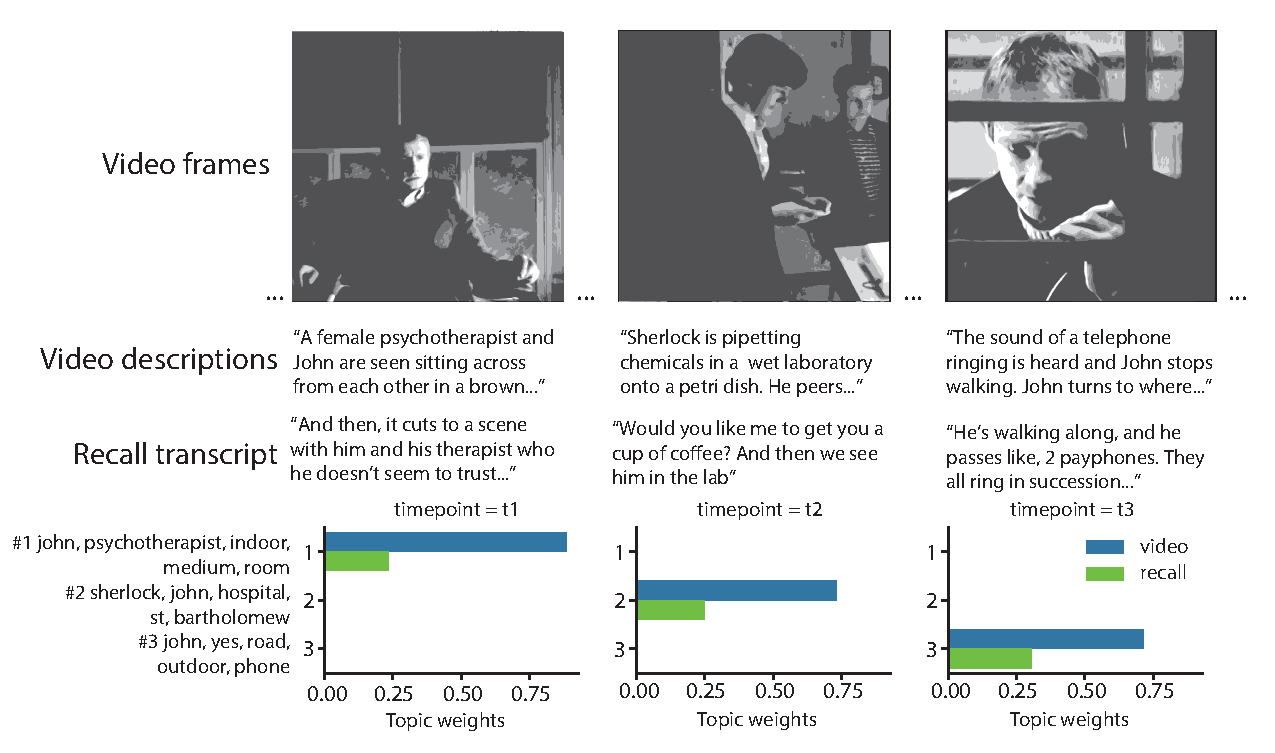
\includegraphics[width=1\textwidth]{figs/analysis_schematic_bw}
\caption{\small \textbf{Methods overview.} We used hand-annotated descriptions of each moment of video to fit a topic model.  Three example video frames, and their associated descriptions are displayed (top two rows).  Participants later recalled the video (in the third row, we show example recalls of the same three scenes from one participant).  We used the topic model (fit to the annotations) to estimate topic vectors for each moment of video and each sentence the participants recalled.  Example topic vectors are displayed in the bottom row (green: video annotations; blue: example participant's recalls).  Three topic dimensions are shown (the highest-weighted topics for each of the three example scenes, respectively).  We also show the 5 highest-weighted words for each topic.  Figure~\topics~provides a full list of the top 10 words from each of the discovered topics.}
\label{fig:schematic}
\end{figure}

The topics we found were heavily character-focused (e.g., the top-weighted word in each topic was nearly always a character) and could be roughly divided into themes that were primarily Sherlock-focused; primarily John-focused (John is Sherlock's close confidant and assistant); or that involved Sherlock and John interacting (Fig.~\topics).  Several of the topics were highly similar, which we hypothesized might allow us to distinguish between subtle narrative differences (if the distinctions between those overlapping topics were meaningful; also see Fig.~\featureimportance).  The topic vectors for each timepoint were \textit{sparse}, in that only a small number (usually one or two) topics tended to be ``active'' in any given timepoint (Fig.~\ref{fig:model}A).  Further, the dynamics of the topic activations appeared to exhibit \textit{persistance} (i.e., given that a topic was active in one timepoint, it was likely to be active in the following timepoint) along with \textit{occasional rapid changes} (i.e., occasionally topics would appear to spring into or out of existence).  These two properties of the topic dynamics may be seen in the block diagonal structure of the timepoint-by-timepoint correlation matrix (Fig.~\ref{fig:model}B).  Following \cite{BaldEtal17}, we used a Hidden Markov Model (HMM) to identify the \textit{event boundaries} where the topic activations changed rapidly (i.e., at the boundaries of the blocks in the correlation matrix; event boundaries identified by the HMM are outlined in yellow).  Part of our model fitting procedure required selecting an appropriate number of ``events'' to segment the timeseries into.  We used an optimization procedure to identify the number of events that maximized within-event stability while also minimizing across-event correlations (see \textit{Methods} for additional details).  To create a stable ``summary'' of the video, we computed the average topic vector within each event (Fig.~\ref{fig:model}C).

\begin{figure}[tp]
\centering
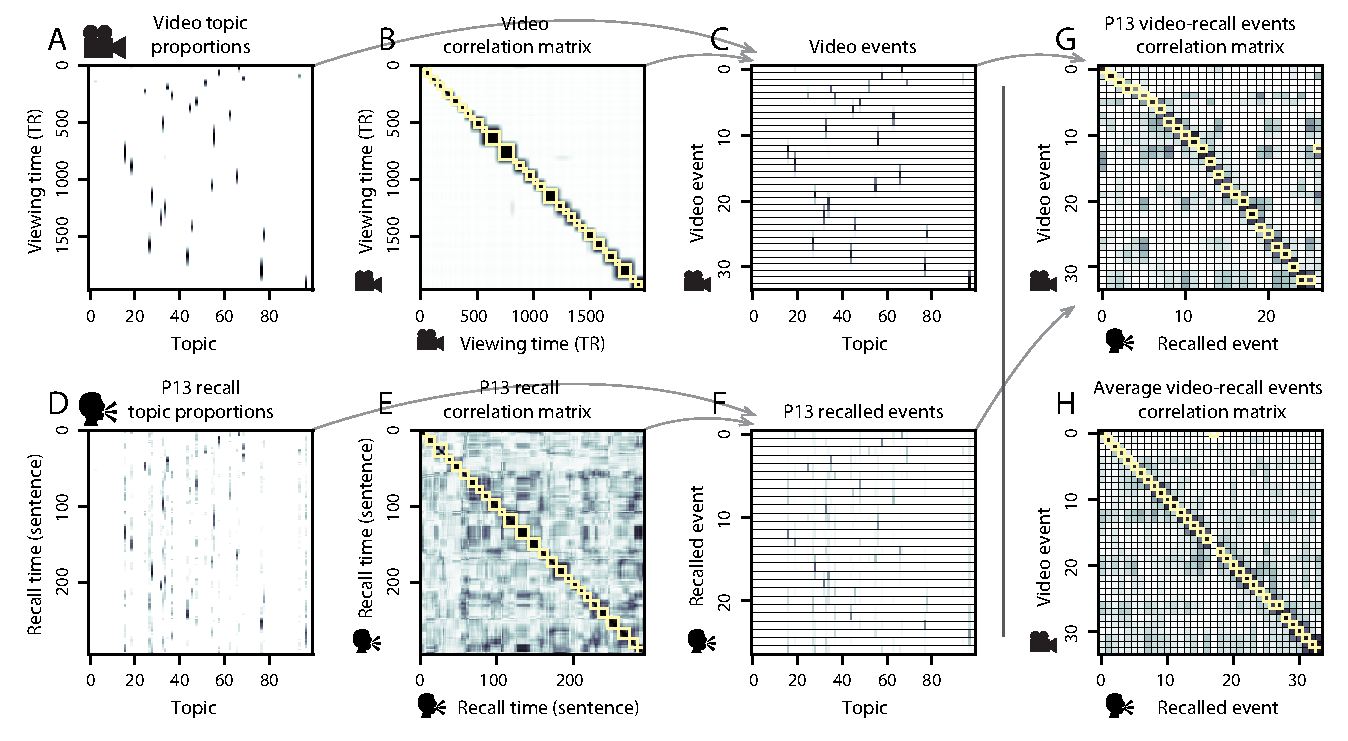
\includegraphics[width=\textwidth]{figs/eventseg}
\caption{\small \textbf{Modelling naturalistic stimuli and recalls.} All panels: darker colors indicate greater values; range: [0, 1].  \textbf{A.} Topic vectors ($K = 100$) for each of the 1976 video timepoints.  \textbf{B.} Timepoint-by-timepoint correlation matrix of the topic vectors displayed in Panel A.  Event boundaries detected by the HMM are denoted in yellow (34 events detected).  \textbf{C.} Average topic vectors for each of the 34 video events. \textbf{D.} Topic vectors for each of 294 sentences spoken by an example participant while recalling the video.  \textbf{E.} Timepoint-by-timepoint correlation matrix of the topic vectors displayed in Panel D. Event boundaries detected by the HMM are denoted in yellow (27 events detected).  \textbf{F.} Average topic vectors for each of the 27 recalled events from the example participant.  \textbf{G.} Correlations between the topic vectors for every pair of video events (Panel C) and recalled events (from the example participant; Panel F).  For similar plots for all participants see Figure~\matchmats.  \textbf{H.} Average correlations between each pair of video events and recalled events (across all 17 participants).  To create the figure, each recalled event was assigned to the video event with the most correlated topic vector.}
\label{fig:model}
\end{figure}

Given that the time-varying content of the video could be segmented cleanly into discrete events, we wondered whether participants' recalls of the video also displayed a similar structure.  We applied the same topic model (already trained on the video annotations) to each participant's recalls.  Analogous to how we analyzed the time-varying content of the video, to obtain similar estimates for participants' recalls we treated each (overlapping) 10 sentence ``window'' of their transcript as a ``document'' and then computed the most probable mix of topics reflected in each timepoint's sentences.  This yielded, for each participant, a number-of-sentences by number-of-topics topic proportions matrix that characterized how the topics identified in the original video were reflected in the participant's recalls.  Note that an important feature of our approach is that it allows us to compare participant's recalls to events from the original video, despite that different participants may have used different language to describe the same event, and that those descriptions may not match the original annotations.  This is a huge benefit of projecting the video and recalls into a shared ``topic'' space.  An example topic proportions matrix from one participant's recalls is shown in Figure~\ref{fig:model}D.

Although the example participant's recall topic proportions matrix has some visual similarity to the video topic proportions matrix, the time-varying topic proportions for the example participant's recalls are not as sparse as for the video (e.g., compare Figs.~\ref{fig:model}A and D).  Similarly, although there do appear to be periods of stability in the recall topic dynamics (e.g., most topics are active or inactive over contiguous blocks of time), the overall timecourses are not as cleanly delineated as the video topics are.  To examine these patterns in detail, we computed the timepoint-by-timepoint correlation matrix for the example participant's recall topic proportions (Fig.~\ref{fig:model}E).  As in the video correlation matrix (Fig.~\ref{fig:model}B), the example partipant's recall correlation matrix has a strong block diagonal structure, indicating that their recalls are discretized into separated events.  As for the video correlation matrix, we can use an HMM, along with the aforementioned number-of-events optimization procedure (also see \textit{Methods}) to determine how many events are reflected in the participant's recalls and where specifically the event boundaries fall (outlined in yellow).  We carried out a similar analysis on all 17 participants' recall topic proportions matrices (Fig.~\corrmats).

Two clear patterns emerged from this set of analyses.  First, although every individual participant's recalls could be segmented into discrete events (e.g.\ every individual participant's recall correlation matrix exhibited clear block diagonal structure; Fig.~\corrmats), each participant appeared to have a unique \textit{recall resolution}, reflected in the sizes of those blocks.  For example, some participants' recall topic proportions segmented into just a few events (e.g.\ Participants 1, 4, and 15), while others' recalls segmented into many shorter duration events (e.g.\ Participants 12, 13, and 17).  This suggests that different participants may be recalling the video with different levels of detail-- e.g. some might touch on just the major plot points, whereas others might attempt to recall every minor scene.  The second clear pattern present in every individual participant's recall correlation matrix is that, unlike in the video correlation matrix, there are substantial off-diagonal correlations in participant's recalls.  Whereas each event in the original video (was largely) separable from the others (Fig.~\ref{fig:model}B), in transforming those separable events into memory participants appear to be integrating \textit{across} different events, blending elements of previously recalled and not-yet-recalled events into each newly recalled event~\citep[Figs.~\ref{fig:model}D, \corrmats; also see][]{MannEtal11, HowaEtal12}.

The above results indicate that both the structure of the original video and participants' recalls of the video exhibit event boundaries that can be identified automatically by characterizing the dynamic content using a shared topic model and segmenting the content into events using HMMs.  Next we asked whether some correspondence might be made between the specific content of the events the participants experienced in the video, and the events they later recalled.  One approach to linking the experienced (video) and recalled events is to label each recalled event as matching the video event with the most similar (i.e., most highly correlated) topic vector (Figs.~\ref{fig:model}G, \matchmats).  This yields a sequence of ``presented'' events from the original movie, and a sequence of (potentially differently ordered) ``recalled'' events for each participant.  Analogous to classic list-learning studies, we can then examine participants' recall sequences by asking which events they tended to recall first~\citep[e.g., probability of first recall; Fig.~\listlearning A; ][]{WelcBurn24, PostPhil65, AtkiShif68}; how participants most often transition between recalls of the events as a function of the temporal distance between them~\citep[e.g., lag-conditional response probability; Fig.~\listlearning B; ][]{Kaha96}; and which events they were likely to remember overall~\citep[e.g., serial position recall analyses; Fig.~\listlearning C; ][]{Murd62a}.  In list-learning studies, this set of three analyses may be used to gain a nearly complete view into the sequences of recalls participants made~\citep[e.g., ][]{Kaha12}.  Extending these analyses to apply to naturalistic stimuli and recall~\citep{HeusEtal17b} highlights that, in naturalistic recall, these analyses provide a wholly incomplete picture: they leave out any attempt to quantify participants' abilities to capture the \textit{content} of what occurred in the video (i.e., their only experimental instruction!).

The dynamic content of the video and participants' recalls is quantified in the corresponding topic proportion matrices.  However, it is difficult to gain deep insights into that content by directly examining the topic proportion matrices (e.g., Figs.~\ref{fig:model}A, D) or the corresponding correlation matrices (Figs.~\ref{fig:model}B, E, \corrmats).  To visualize the time-varying high-dimensional content in a more intuitive way~\citep{HeusEtal18} we projected the topic proportion matrices onto a two-dimensional space using Uniform Manifold Approximation and Projection~\citep[UMAP; ][]{McInHeal18}.  In this lower-dimensional space, each point represents a single video or recall event, and the distances between the points reflect the distances between the events' associated topic vectors (Fig.~\ref{fig:trajectory}).

\begin{figure}[tp]
\centering
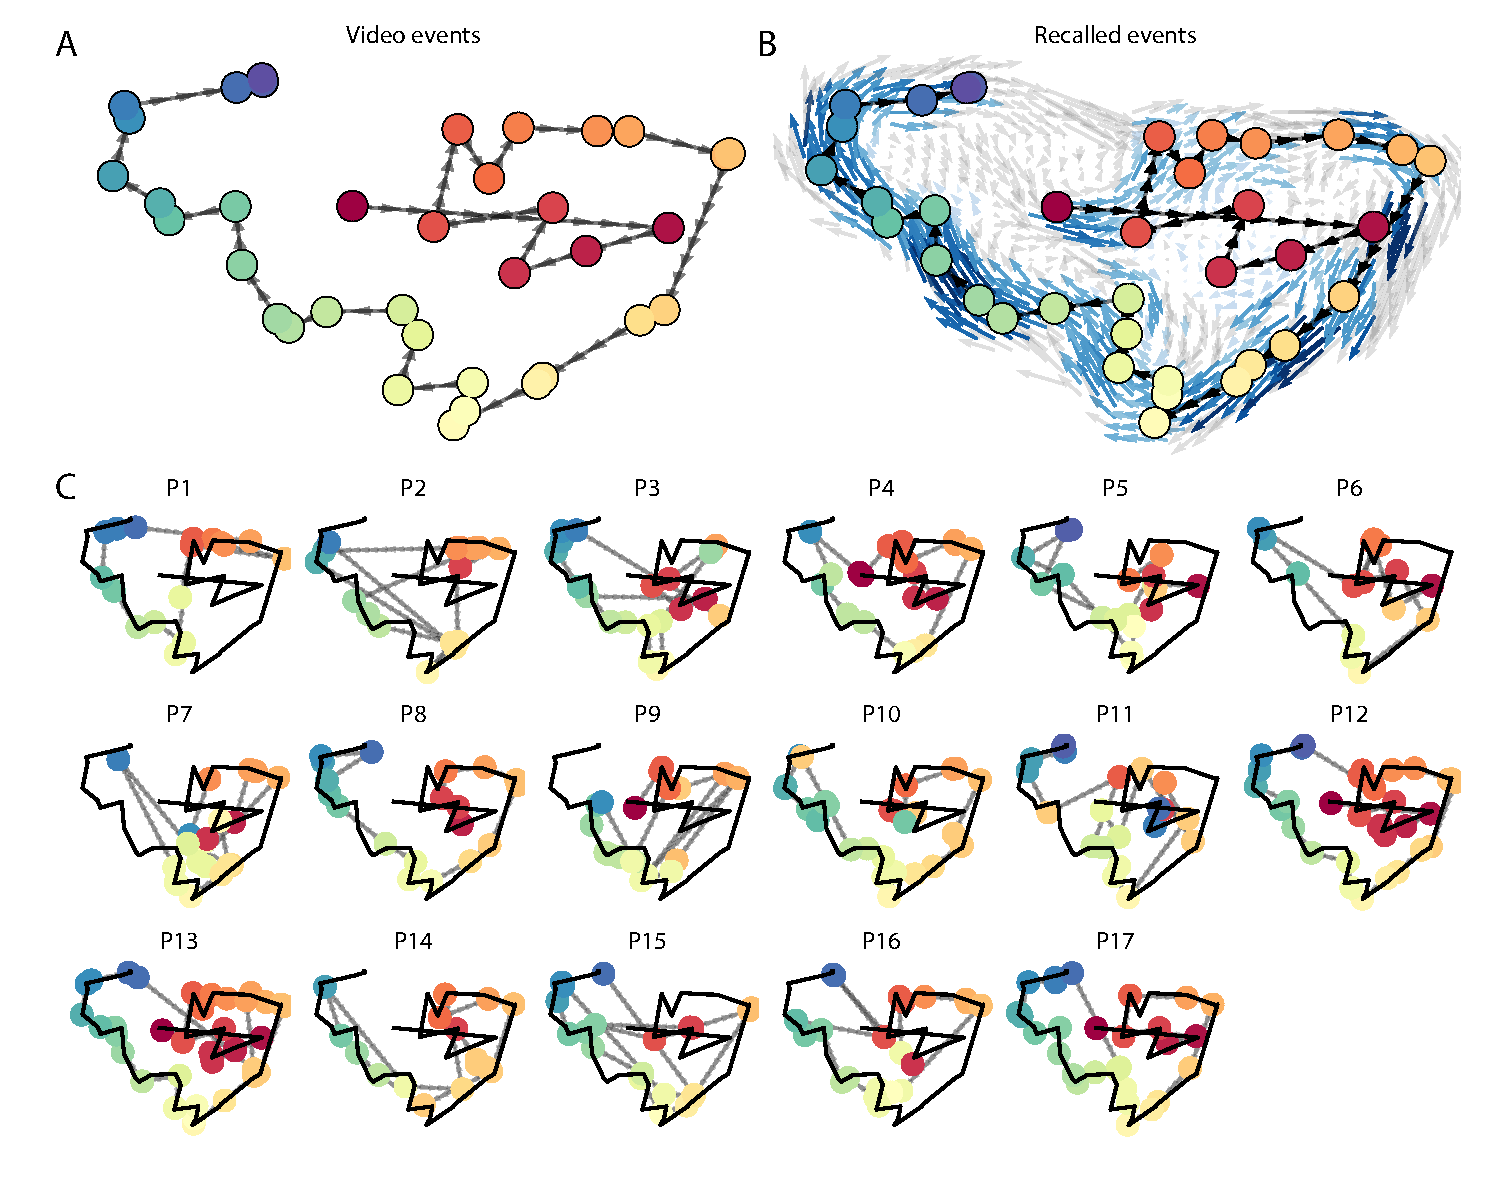
\includegraphics[width=1\textwidth]{figs/trajectory}
\caption{\small \textbf{Trajectories through topic space capture the dynamic content of the video and recalls.}  All panels: the topic proportion matrices have been projected onto a shared two-dimensional space using UMAP.  \textbf{A.} The two-dimensional topic trajectory taken by the episode of \textit{Sherlock}.  Each dot indicates an event identified using the HMM (see \textit{Methods}); the dot colors denote the order of the events (early events are in red; later events are in blue), and the connecting lines indicate the transitions between successive events.  \textbf{B.} The average two-dimensional trajectory captured by participants' recall sequences, with the same format and coloring as the trajectory in Panel A.  To compute the event positions, we matched each recalled event with an event from the original video (see text), and then we averaged the positions of all events with the same label.  The arrows reflect the average transition direction through topic space taken by any participants whose trajectories crossed that part of topic space; blue denotes reliable agreement across participants via a Rayleigh test ($p < 0.05$, corrected).  \textbf{C.} The recall topic trajectories taken by each individual participant (1--17).  The video's trajectory is shown in black for reference.  (Same format and coloring as Panel A.)}
\label{fig:trajectory}
\end{figure}

Visual inspection of the video and recall topic trajectories reveals a striking pattern.  First, the topic trajectory of the video (which reflects its dynamic content; Fig.~\ref{fig:trajectory}A) is captured nearly perfectly by the averaged topic trajectories of participants' recalls (Fig.~\ref{fig:trajectory}B).  To assess the consistency of these recall trajectories across participants, we asked: given that a participant's recall trajectory had entered a particular location in topic space, could the position of their \textit{next} recalled event be predicted reliably?  For each location in topic space, we computed the set of line segments connecting successively recalled events (across all participants) that intersected that location (see \textit{Methods} for additional details).  We then computed (for each location) the distribution of angles formed by the lines defined by those line segments and a fixed reference line (the $x$-axis).  Rayleigh tests revealed the set of locations in topic space at which these across-participant distributions exhibited reliable peaks (blue arrows in Fig.~\ref{fig:trajectory}B).  We observed that the locations traversed by nearly the entire the video trajectory exhibited such peaks.  In other words, participants exhibited similar trajectories that also matched the trajectory of the original video (Fig.~\ref{fig:trajectory}C).  This is especially notable when considering the fact that the number of events participants recalled (dots in Fig.~\ref{fig:trajectory}C) varied considerably across people, and that every participant used different words to describe what they had remembered happening in the video.  Differences in the numbers of remembered events appear in participants' trajectories as differences in the sampling resolution along the trajectory.  We note that this framework also provides a means of detangling classic ``proportion recalled'' measures (i.e., the proportion of video events referenced in participants' recalls) from participants' abilities to recaputulate the full gist of the original video (i.e., the similarity in the shape of the original video trajectory and that defined by each participant's reocounting of the video).

Because our analysis framework projects the dynamic video content and participants' recalls onto a shared topic space, and because the dimensions of that space are known (i.e., each topic dimension is a set of weights over words in the vocabulary; Fig.~\topics), we can examine the topic trajectories to understand which specific content was remembered well (or poorly).  For each video event, we can ask: what was the average correlation (across participants) between the video event's topic vector and the closest matching recall event topic vectors from each participant? This yields a single correlation coefficient for each video event, describing how closely participants' recalls of the event tended to reliably capture its content (Fig.~\ref{fig:topics}A).  (We also examined how different comparisons between each video event's topic vector and the corresponding recall event topic vectors related to hand-annotated characterizations of memory performance; see \textit{Supplemental Materials}).  Given this summary of which events were recalled reliably (or not), we next asked whether the better-remembered or worse-remembered events tended to reflect particular topics.  We computed a weighted average of the topic vectors for each video event, where the weights reflected how reliably each event was recalled.  To visualize the result, we created a ``wordle'' image~\citep{MuelEtal18} where words weighted more heavily by better-remembered topics appear in a larger font (Fig.~\ref{fig:topics}B, green box).  Events that reflected topics weighting heavily on characters like ``Sherlock'' and ``John'' (i.e., the main characters) and locations like ``221b Baker Street'' (i.e., a major recurring location; the address of the flat that Sherlock and John share) were best remembered.  An analogous analysis revealed which themes were poorly remembered; here in computing the weighted average over events' topic vectors we weighted each event in \textit{inverse} proportion to how well it was remembered (Fig.~\ref{fig:topics}B, red box).  This revealed that events with relatively minor characters such as ``Mike,'' ``Jeffrey,'' and ``Molly,'' as well as less-integral plot locations (e.g., ``hospital'' and ``office'') were least well-remembered.  This suggests that what is retained in memory are the major plot elements (i.e., the overall ``gist'' of what happened), whereas the more minor details are prone to pruning.

In addition to constructing overall summaries, assessing the video and recall topic vectors from individual recalls can provide further insights.  Specifically, for any given event we can construct a wordle from that event's topic vector, and we can construct a similar wordle from the average topic vectors produced by all participants who recalled that event.  We can then examine those wordles visually to gain an intuition for which aspects of the video event were recapitulated in participants' recalls of that event.  Several example wordles are displayed in Figure~\ref{fig:topics}C (wordles from the three best-remembered events are circled in green; wordles from the three worst-remembered events are circled in red).  Using wordles to visually compare the topical content of each video event and the (average) corresponding recall event reveals the specific content from the specific events that is reliably retained in the transformation into memory (green events) or not (red events).

\begin{figure}[tp]
\centering
\includegraphics[width=1\textwidth]{figs/topics}
\caption{\small \textbf{Transforming experience into memory.} \textbf{A.} Average correlations (across participants) between the topic vectors from each video event and the closest-matching recall events.  Error bars denote bootstrap-derived across-participant 95\% confidence intervals.  The stars denote the three best-remembered events (green) and worst-remembered events (red).  \textbf{B.} Wordles comprising the top 200 highest-weighted words reflected in the weighted-average topic vector across video events.  Green: video events were weighted by how well the topic vectors derived from recalls of those events matched the video events' topic vectors (Panel A).  Red: video events were weighted by the inverse of how well their topic vectors matched the recalled topic vectors.  \textbf{C.}  The set of all video and recall events is projected onto the two-dimensional space derived in Figure~\ref{fig:trajectory}.  The dots outlined in black denote video events (dot size reflects the average correlation between the video event's topic vector and the topic vectors from the closest matching recalled events from each participant; bigger dots denote stronger correlations).  The dots without black outlines denote recalled events.  All dots are colored using the same scheme as Figure~\ref{fig:trajectory}A.  Wordles for several example events are displayed (green: three best-remembered events; red: three worst-remembered events).  Within each circular wordle, the left side displays words associated with the topic vector for the video event, and the right side displays words associated with the (average) recall event topic vector, across all recall events matched to the given video event.}
\label{fig:topics}
\end{figure}

The results thus far tell us about which aspects of the dynamic content in the episode participants watched were preserved or altered in participants' memories of the episode.  We next carried out a series of analyses aimed at understanding which brain structures might implement these processes.  In one analysis we sought to identify which brain structures were sensitive to the video's dynamic content, as characterized by its topic trajectory.  Specifically, we used a searchlight procedure to identify the extent to which each cluster of voxels exhibited a timecourse (as the participants watched the video) whose temporal correlation matrix matched the temporal correlation matrix of the original video's topic proportion matrix (Fig.~\ref{fig:model}B).  As shown in Figure~\ref{fig:brainz}A, the analysis revealed a network of regions including bilateral frontal and cingulate cortex, suggesting that these regions may play a role in maintaining information relevant to the narrative structure of the video.  In a second analysis, we sought to identify which brain structures' responses (while viewing the video) reflected how each participant would later \textit{recall} the video.  Specifically, we used an analogous searchlight procedure to identify clusters of voxels whose temporal correlation matrices reflected the temporal correlation matrix of the topic proportions for each individual's recalls (Figs.~\corrmats).  As shown in Figure~\ref{fig:brainz}B, the analysis revealed a network of regions including the ventromedial prefrontal cortex (vmPFC), anterior cingulate, and right medial temporal lobe (rMTL), suggesting that these regions may play a role in transforming each individual's experience into memory.

\begin{figure}[tp]
\centering
\includegraphics[width=1\textwidth]{figs/brains_panels}
\caption{\small \textbf{Brain structures that underlie the transformation of experience into memory.} \textbf{A.} We searched for regions whose responses (as participants watched the video) matched the temporal correlation matrix of the video topic proportions.  These regions are sensitive to the narrative structure of the video.  \textbf{B.} We searched for regions whose responses (as participants watched the video) matched the temporal correlation matrix of the topic proportions derived from each individual's later recall of video.  These regions are sensitive to how the narrative structure of the video is transformed into a memory of the video.  Both panels: the maps are thresholded at $p < 0.05$, corrected.}
\label{fig:brainz}
\end{figure}


\section*{Discussion}
\label{sec:discussion}

One approach to identifying neural responses to naturalistic stimuli (including experiences) entails building a model of the stimulus and searching for brain regions whose responses are consistent with the model.  In prior work, a series of studies from Uri Hasson's group~\citep{LernEtal11, SimoEtal16, ChenEtal17, BaldEtal17, ZadbEtal17} have extended this approach with a clever twist.  Rather than building an explicit stimulus model, these studies instead search for brain responses (while experiencing the stimulus) that are reliably similar across individuals.  So called \textit{inter-subject correlation} (ISC) and \textit{inter-subject functional connectivity} (ISFC) analyses effectively treat other people's brain responses to the stimulus as a ``model'' of how its features change over time.  By contrast, in our present work we used topic models and HMMs to construct an explicit stimulus model (i.e., the topic trajectory of the movie).  When we searched for brain structures whose responses are consistent with the video's topic trajectory, we identified a network of structures that overlaped strongly with the ``long temporal receptive window'' network reported by the Hasson group~\citep[e.g., compare our Fig.~\ref{fig:brainz}A with the map of long temporal receptive window voxels in][]{LernEtal11}.  This provides support for the notion that part of the long temporal receptive window network may be maintaining an explicit model of the stimulus dynamics.  When we performed a similar analysis after swapping out the video's topic trajectory with the recall topic trajectories of each individual participant, this allowed us to identify brain regions whose responses (as the participants viewed the video) reflected how the video trajectory would be transformed in memory (as reflected by the recall topic trajectory).  The analysis revealed that the rMTL and vmPFC may play a role in this person-specific transformation from experience into memory.  The role of the MTL in episodic memory encoding has been well-reported~\citep[e.g., ][]{PallWagn02, DavaEtAl03, RangEtal04, Dava06}.  Prior work has also implicated the medial prefrontal cortex in representing ``schema'' knowledge~\citep[i.e., general knowledge about the format of an ongoing experience given prior similar experiencs; ][]{KestEtal12, GilbMarl17}.  Integrating across our study and this prior work, one interpretation is that the person-specific transformations mediated (or represented) by the rMTL and vmPFC may reflect schema knowledge being leveraged, formed, or updated, incorporating ongoing experience into previously acquired knowledge.

Our work has broad implications for how we characterize and assess memory in real-world settings such as the classroom or physician's office.  For example, the most commonly used classroom evaluation tools involve computing the proportion of correctly answered exam questions.  Our work indicates that this approach is only loosly related to what educators might really want to measure: how well did the students understand the key ideas presented in the course?  One could apply the computational framework we developed to construct topic trajectories for the video and participants' recalls to build explicit content models of the course material and exam questions.  This approach would provide a more nuanced and specific view into which aspects of the material students had learned well (or poorly).  In clinical settings, memory measures that incorporate such explicit content models might also provide more direct evaluations patients' memories.




\section*{Methods}
\label{sec:methods}

\subsection*{Participants and Experimental Design}
Data were collected by \cite{ChenEtal17}.  In brief, participants ($n=17$) viewed the first 48 minutes of ``A Study in Pink'', the first episode of the BBC television series \textit{Sherlock}, while fMRI volumes were collected (TR = 1500~ms).  The stimulus was divided into a 23 minute and a 25 minute segment to facilitate technical issues related to the scanner.  After finishing the clip, participants were instructed to \citep[quoting from][]{ChenEtal17} ``describe what they recalled of the movie in as much detail as they could, to try to recount events in the original order they were viewed in, and to speak for at least 10 minutes if possible but that longer was better. They were told that completeness and detail were more important than temporal order, and that if at any point they realized they had missed something, to return to it. Participants were then allowed to speak for as long as they wished, and verbally indicated when they were finished (e.g., `I’m done').''  For additional details about the experimental procedure and scanning parameters see \cite{ChenEtal17}.

\subsection*{Modeling the dynamic content of the video and recall transcripts}
\subsubsection*{Topic modeling}
The input to the topic model we trained to characterize the dynamic content of the video comprised hand-generated annotations of each of 1000 scenes spanning the video clip~\citep[generated by][]{ChenEtal17}.  The features included: narrative details (a sentence or two describing what happened in that scene); whether the scene took place indoors or outdoors; names of any characters that appeared in the scene; name(s) of characters in camera focus; name(s) of characters who were speaking in the scene; the location (in the story) that the scene took place; camera angle (close up, medium, long, top, tracking, over the shoulder, etc.); whether music was playing in the scene or not; and a transcription of any on-screen text.  We concatenated the text for all of these features within each segment, creating a ``bag of words'' describing each scene.  We then re-organized the text descriptions into overlapping sliding windows spanning 50 scenes each. In other words, the first text sample comprised the combined text from the first 50 scenes (i.e., 1--50), the second comprised the text from scenes 2--51, and so on.  We trained our model using these overlapping text samples with \texttt{scikit-learn}~\citep[version 0.19.1; ][]{PedrEtal11}, called from our high-dimensional visualization and text analysis software, \texttt{HyperTools}~\citep{HeusEtal18}.  Specifically, we use the \texttt{CountVectorizor} class to transform the text from each scene into a vector of word counts (using the union of all words across all scenes as the ``vocabulary,'' excluding English stop words); this yields a number-of-scenes by number-of-words \textit{word count} matrix.  We then use the \texttt{LatentDirichletAllocatin} class (topics=100, method=`batch') to fit a topic model~\citep{BleiEtal03} to the word count matrix, yielding a number-of-scenes (1000) by number-of-topics (100) \textit{topic proportions} matrix.  The topic proportions matrix describes which mix of topics (latent themes) is present in each scene.  Next, we transformed the topic proportions matrix to match the 1976 fMRI volume acquisition times.  For each fMRI volume, we took the topic proportions from whatever scene was displayed for most of that volume's 1500~ms acquisition time.  This yielded a new number-of-TRs (1976) by number-of-topics (100) topic proportions matrix.

We created similar topic proportion matrices using hand-annotated transcripts of each participant's recall of the video~\citep[annotated by ][]{ChenEtal17}.  We tokenized the transcript into a list of sentences, and then re-organized the list into overlapping sliding windows spanning 10 sentences each; we in turn transformed each window's sentences into a word count vector (using the same vocabulary as for the video model).  We then used the topic model already trained on the video scenes to compute the most probable topic proportions for each sliding window.  This yielded a number-of-sentences (range: 68--294) by number-of-topics (100) topic proportions matrix, for each participant.  These reflected the dynamic content of each participant's recalls.  Note: for details on how we selected the video and recall window lengths and number of topics, see \textit{Supplemental Materials} and Figure~\topicopt.


\textbf{JRM STOPPED HERE}

\subsubsection*{Extracting events using a hidden Markov model}
The topic model timepoint-by-timepoint correlation matrices all exhibited a block-diagonal structure (with small off-diagonal values), suggesting that the models were comprised of a number of sequential `states' (or events, see Fig.~\corrmats). To capture this structure, we fit the video and each recall model using a hidden Markov model (HMM). Given a number of states or events ($k$), the HMM recovers a set of labels that segments consecutive timepoints into $k$ events ~\citep{Rabi89, BaldEtal17}. To implement this analysis, we used the BrainIAK toolbox \citep{BaldEtal17, Brainiak}.

Our metric for choosing the ``best fitting'' HMM was to choose the model with the $k$ value that maximized the ratio of the average `within-event' correlation values (i.e., the correlation values for blocks of consecutive timepoints the model identified as one event) and the average `across-event' correlation (i.e., the rest of the correlation values). Additionally, we included a penalty parameter that was proportional to the smoothing of the model that preferred models with smaller $k$ values. We chose $k$ values separately for the video model and for each recall model.  Then, using the best $k$ values, We fit a separate HMM for the video and each recall model. Finally, we averaged over timepoints identified to be in the same event resulting in a events by topics matrix for the video model and each of the recall models.

\subsubsection*{Matching recall events to video events}
To estimate which video event each recall event referred to, we correlated the video events model and each recall events model. This resulted in a video events (34) by recall events (8-27) correlation matrix (for each participant) which contains the similarity between each video event and each recall event (see Fig.~\matchmats).  To find the most likely video event that a given recall event referred to, we computed the argmax over the columns of this matrix.  The result was a list of video event indices for each participant. These indices are analogous to the values found in a ``recall matrix'' from a free recall list learning experiment, but represent the recall of particular events (instead of words, for example).

\subsubsection*{Visualizing the video and recall event models}
To visualize the temporal structure of the video event model (34 events by 100 topics) and the recall event models (8-27 events by 100 topics), we used a technique called UMAP ~\citep{McInHeal18} to reduce the ``topic-space'' from 100 dimensions down to 2 dimensions. UMAP is a nonlinear dimensionality reduction technique which models the manifold of the data with a fuzzy topological structure, and then searches for a (2D) projection of the data that has the closest equivalent fuzzy topological structure. We concatenated (vertically stacked) all event models (video, average recall, and individual recall), and then fit and transformed all of the models at once. This assured that the models were projected into the same space.

\subsubsection*{Vector field analysis}
To quantify the flow of recall from event to event, we performed a vector field analysis.  We tiled the 2D topic space (x, y: -6 to 6 by .25) with an evenly spaced grid. For each grid point, we drew a circle around the point (radius= 0.5). Then, we tested whether any line segments (formed by event recall transitions) passed through this area of the topic space.  For example, say that a participant transitioned from recalling event 2 to event 3. These 2 recall events correspond to 2 points in topic space, and connecting them forms a line segment. We collected all line segments that passed through a given section of topic space (collapsing across participants). To plot the average direction of the line segments (i.e., the arrows for each grid point in Fig.~\ref{fig:trajectory}B), we converted each of them to unit vectors and then averaged. For grid points where the direction was consistent (across all participants contributing to that point), the length of the arrow approaches 1, whereas if the direction was random the length of the arrow approaches 0. Lastly, we converted each unit vector to an angle (in radians) by taking the inverse tangent of the x, y components of the vector. To test whether the distribution of angles was significantly non-uniform (i.e., displayed a preferred direction across participants), we performed a Rayleigh test on the angles ($p < 0.001$, FDR-corrected at $p < 0.05$ using Benjamani-Hochberg procedure). Arrows where the Rayleigh test was significant are displayed in color (the darker the blue the more significant) while non-significant tests are displayed in gray with lower opacity.

\subsubsection*{Topic vector word clouds}
We created word clouds to visualize the themes contained in the recall events. One component of the topic model comprises a words (2117) by topics (100) matrix (R), where the rows represent the weight of a given word in each topic.  To find words that were maximally associated with a particular event vector, we computed the dot product between R and v, which gave a 1 by \# of words vector where the values represent the ``activation'' of each of in the event. Activation is defined as the weight of a particular word in a particular event. Then, we created word clouds by extracting the top $n$ words and plotting them where the size of the word is proportional to its activation in the event.

In the first analysis (Fig.~\ref{fig:topics}A,B), we quantified the most and least remembered topics/words throughout the entire video by computing a weighted average over all recall events, where the weights were proportional to memory for each recall event. To measure memory for each event, for each participant we computed the correlation between the video event vector and the closest recall event vector. We then averaged these correlation values across participants. We then computed a weighted average of all video events using the correlation values as weights. Next, we computed the dot product between this weighted-average video event vector and the R matrix (described in the paragraph above) to get activations for each word. Finally, we plotted the top 200 words where the size of the word is proportional to its activation. To get the least remembered topics/words, we performed the same analysis but inverted memory weights.

In the second analysis (Fig.~\ref{fig:topics}C), we created wordles for the top/bottom 3 remembered video events indexed by the average correlation values (Fig.~\ref{fig:topics}A).  To get the ``activations'' for words associated with the video events, we computed the dot product between the video event vector and the R matrix. The same procedure was used to get word activations for the recall events. We then plotted the top 200 words for the top/bottom 3 recalled events.

\subsection*{fMRI analyses}
Participants viewed and recalled the video stimulus inside an fMRI scanner. The video was split into two parts of approximately equal length (946 and 1030 TRs, $TR=1.5 seconds$). All data were preprocessed and transformed to 3mm MNI space as described in ~\citep{ChenEtal17}. Data were z-scored across time at every voxel. 6mm smoothing was applied.
Files are cropped so that all video-viewing data are aligned across participants, and all recall data are aligned to the scene timestamps below. The cropping includes a constant 3-TR (4.5 sec) shift to correct for hemodynamic lag.

\subsubsection*{Searchlight analysis}
Our multivariate analyses were designed to capture brain regions whose timepoint-by-timepoint correlational structure mirrors the correlational structure of the video model as well as participant-specific recall topic models during video viewing. We conducted a searchlight analysis (5x5x5 voxel cube) where for each cube, we correlated the model timepoint-by-timepoint correlation matrix with the neural correlation matrix. To aggregate across participants, we Fisher's z-transformed the correlations and then averaged.  To assess significance, we recomputed this group analysis 100 times, but randomly phase shifted the model by the same amount for each participant but different amounts for each permutation to build a null distribution of correlation values. Finally, we thresholded the group averaged correlation maps where the `real' correlation value for a given voxel exceeded the 95th percentile of the null distribution. To correct for non-linearities between the viewing time and recall time, for each participant we used dynamic time warping to temporally align the matrices. The algorithm recovers a path of coordinates that would bring the video and recall model in maximal temporal alignment. We used this path to warp the fMRI data and the recall model into temporal alignment (separately for each participant).


\bibliography{memlab}

\end{document}
